\section{Autoparametric Oscillator Solutions}

In this section, solutions for the autoparametric oscillator system are produced. The first set of solutions is shown in Figures \ref{f:fpe_sigma_1_area_100}, \ref{f:fpe_sigma_1_area_50} and \ref{f:fpe_sigma_1_area_10}. Physical parameters are kept the same for all of the solutions shown with the difference between the Figures being that different maximum areas for the elements are specified. The intent of these Figures is to demonstrate that across the gluing edge, where the finite element method must be formulated carefully, the solution does not exhibit any singularities. As the Figures show, the solutions appear to be continuous across the gluing edge, as expected based on analytic calculations.

\begin{figure}
\begin{center}
\psfrag{H}{$y_1$}
\psfrag{I}{$y_2$}
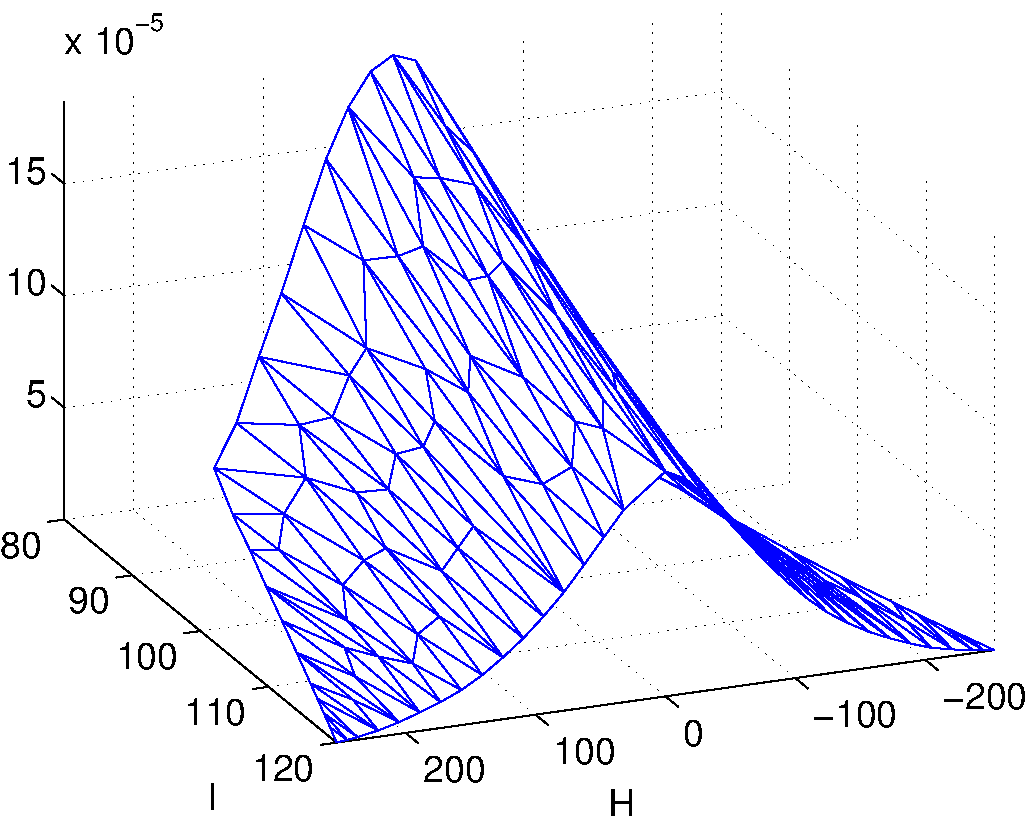
\includegraphics[width=\textwidth]{figures/fpe_solution_sigma_1_area_100}
\caption{Steady-state solution to the FPE obtained by the finite-element method when the maximum element area is 100.}
\label{f:fpe_sigma_1_area_100}
\end{center}
\end{figure}

\begin{figure}
\begin{center}
\psfrag{H}{$y_1$}
\psfrag{I}{$y_2$}
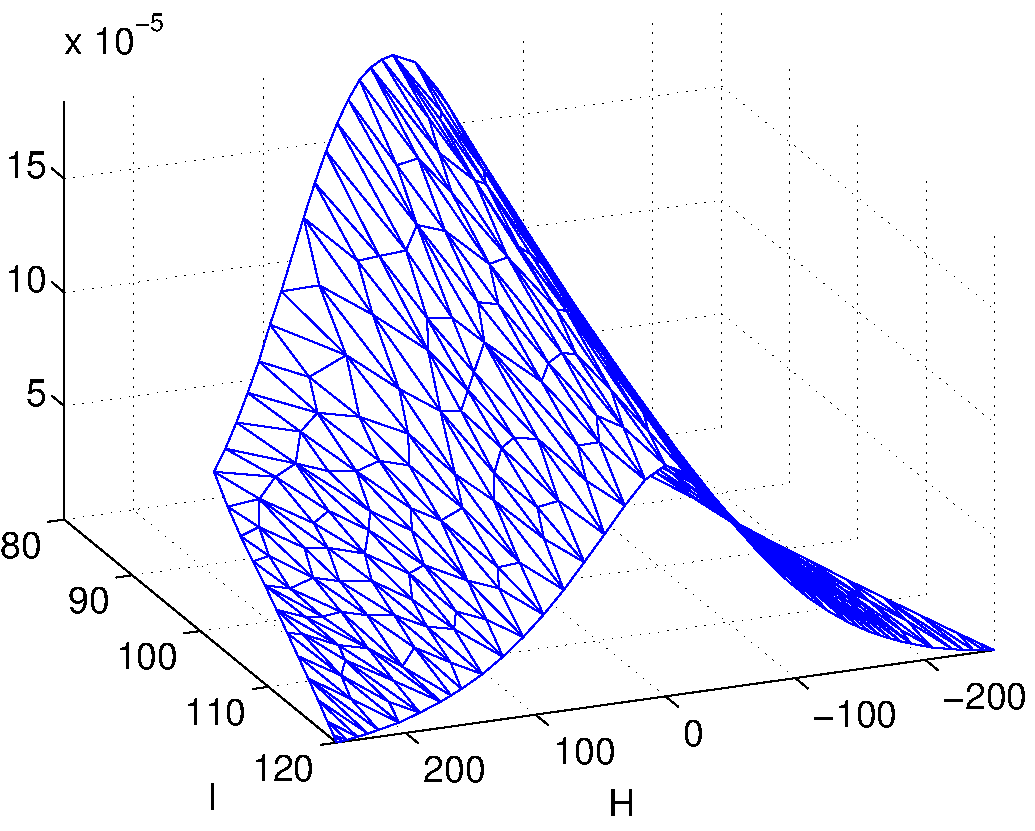
\includegraphics[width=\textwidth]{figures/fpe_solution_sigma_1_area_50}
\caption{Same solution as Figure \ref{f:fpe_sigma_1_area_100}, but with the maximum element area set to 50.}
\label{f:fpe_sigma_1_area_50}
\end{center}
\end{figure}

\begin{figure}
\begin{center}
\psfrag{H}{$y_1$}
\psfrag{I}{$y_2$}
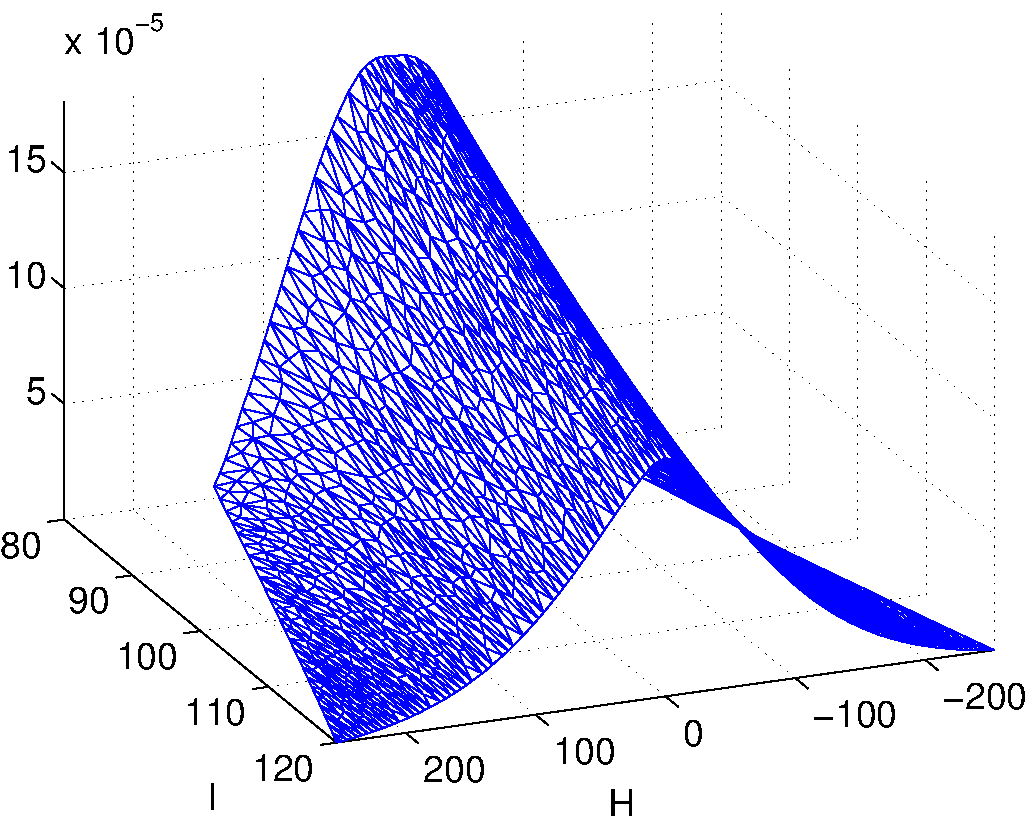
\includegraphics[width=\textwidth]{figures/fpe_solution_sigma_1_area_10}
\caption{Same solution as Figure \ref{f:fpe_sigma_1_area_100}, but with the maximum element area set to 10.}
\label{f:fpe_sigma_1_area_10}
\end{center}
\end{figure}

The next set of results is in shown in Figure \ref{f:fpe_sigma_1_i_lim}. These Figures probe the effect of varying the value of $I_\text{min}$. Recalling that the domain of the FPE has a cusp at the origin, the behavior of the solution near the origin is of interest. In Figure \ref{f:fpe_sigma_1_i_lim}, the FEM solution is plotted along the $I$-axis. Curves in that figure suggest that as the cusp is approached, the solution goes to zero.

\begin{figure}
\begin{center}
\psfrag{I}{$y_2$}
\psfrag{p}{$p$}
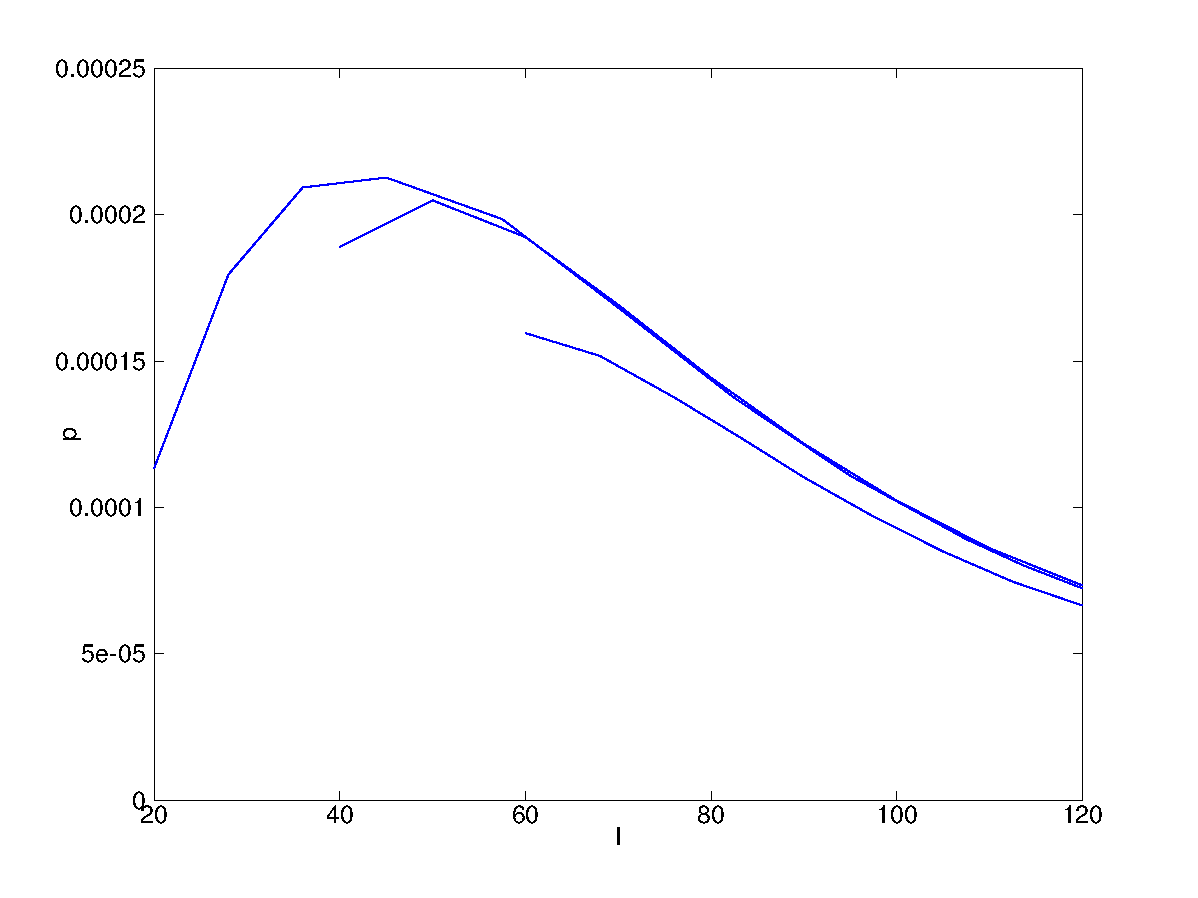
\includegraphics[width=\textwidth,clip=true,viewport=10 10 570 420]{figures/autoparam/i_lim}
\caption{Steady-state solution to the FPE along $y_1$ = 0 for different values of $y_{2,\text{min}}=20,40,60$. It is conjectured that the lines do not overlap exactly due to discretization errors.}
\label{f:fpe_sigma_1_i_lim}
\end{center}
\end{figure}

The final set of solutions is shown in Figures \ref{f:fpe_sigma_.5} and \ref{f:fpe_sigma_1.5}. These figures use the same mesh as Figure \ref{f:fpe_sigma_1_area_50}, but now a physically significant parameter, the amplitude of stochastic forcing, is varied. Although there seems to be a bug in the FEM solver that causes irregularities in the solution near the gluing edge, the overall trend in the solutions seems clear. As forcing amplitude is increased, the peak of the probability distribution moves to larger values of $I$ while remaining symmetric about the $I$ axis. The latter fact is worth contemplating. Recalling the structure of the Hamiltonian, (see Figure \ref{f:autoparam Hamiltonian}) the outer edge of the domain in the left hand plane corresponds to a sink and the outer edge of the domain in the right hand plane is a valley. As such it seems reasonable to think that as forcing amplitude increases, the peak of the PDF will shift from the left hand plane to the right hand plane, but this is not observed in the Figures. In fact, simply by looking at the form of $\mathfrak b_1$ (see Equations \eqref{e:b1 valley} and \eqref{e:b1 hill} and Figure \ref{F:b1_circ}), one notices that along the $K$ axis, the drift coefficient tends to center the probability density on the $I$ axis. It is curious that $\mathfrak b_1$ does not contain any stochastic effects; whether this is a generic feature for systems in 1:2 resonance remains to be determined.

\begin{figure}
\begin{center}
\psfrag{H}{$y_1$}
\psfrag{I}{$y_2$}
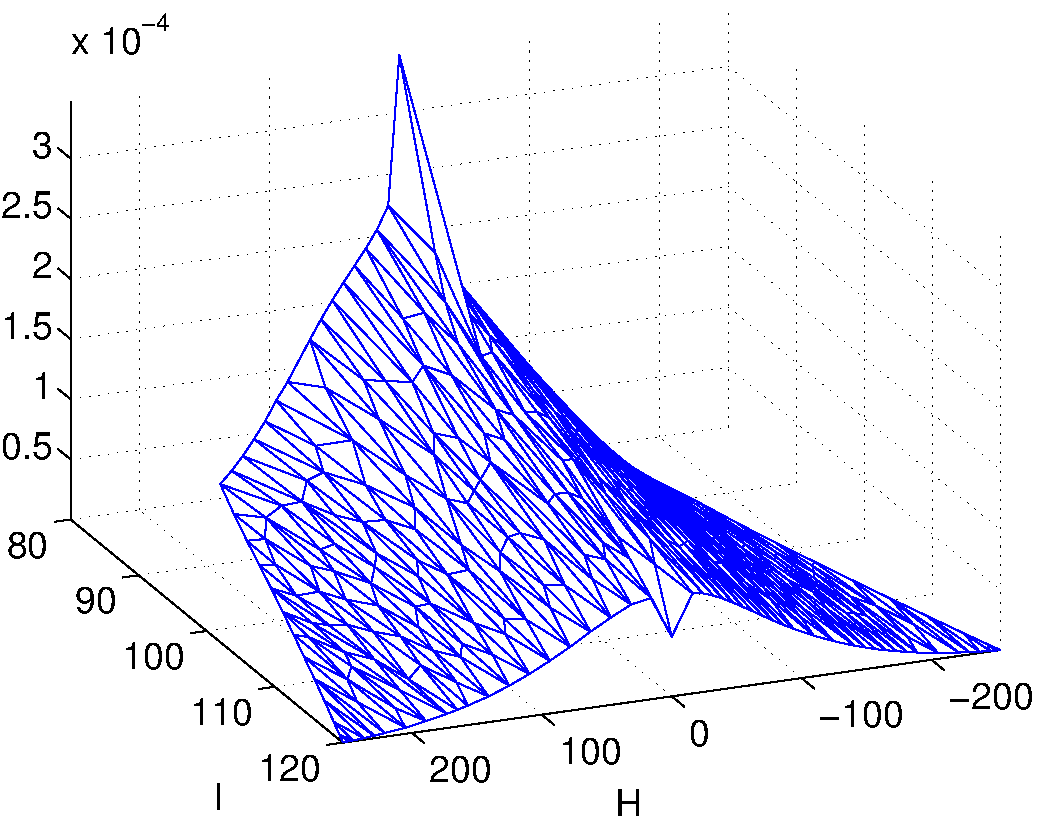
\includegraphics[width=\textwidth]{figures/fpe_solution_sigma_p5}
\caption{Steady-state solution to the FPE obtained by the finite-element method for $\sigma = 0.5$.}
\label{f:fpe_sigma_.5}
\end{center}
\end{figure}

\begin{figure}
\begin{center}
\psfrag{H}{$y_1$}
\psfrag{I}{$y_2$}
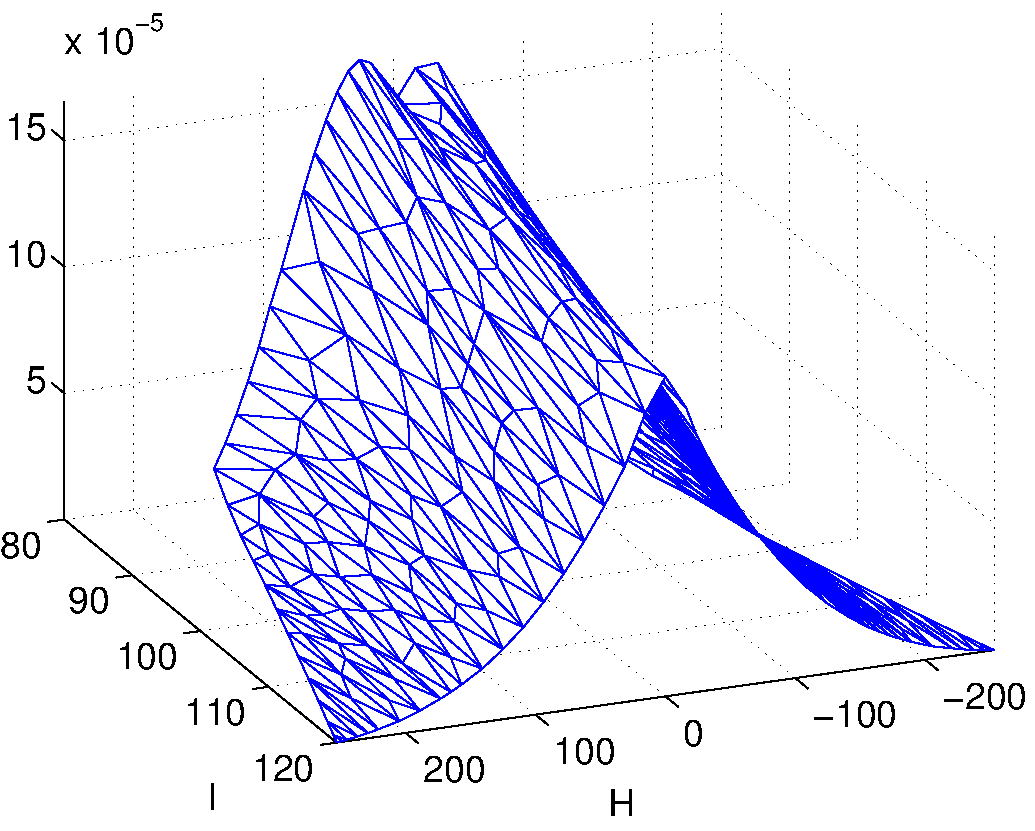
\includegraphics[width=\textwidth]{figures/fpe_solution_sigma_1p5}
\caption{Steady-state solution to the FPE obtained by the finite-element method for $\sigma = 1.5$.}
\label{f:fpe_sigma_1.5}
\end{center}
\end{figure}
